\documentclass{beamer}
\usepackage[utf8]{inputenc}
\usepackage[spanish]{babel}
\usepackage{graphicx}
\usepackage{booktabs}
\usepackage{listings}
\usepackage{amsmath}

\usetheme{Madrid}

\title{Cuantificación: Estimación de Prevalencias por Clase}
\subtitle{Taller práctico}
\author{[Pablo González, Olaya Pérez-Mon]}
\institute{[Universidad de Oviedo]}
\date{\today}

\setbeamertemplate{footline}{}
\begin{document}

\begin{frame}
    \titlepage
    \vfill
    \centering
    \begin{minipage}[c]{0.3\textwidth}
        
\includegraphics[width=\linewidth]{images/logo.png}
    \end{minipage}
    \hspace{1cm}
    \begin{minipage}[c]{0.3\textwidth}
        
\includegraphics[width=\linewidth]{images/aepia.png}
    \end{minipage}
\end{frame}


% 1. Introducción
\begin{frame}{Objetivos del taller}
\begin{itemize}
    \item Poner en práctica los conceptos vistos en la sesión teórica: \textit{Cuantificación, estimación de prevalencias por clase mediante aprendizaje supervisado.}
    \item Entender cuando necesitamos la cuantificación desde un enfoque práctico.
    \item Introducir herramientas para implementar cuantificadores de forma sencilla (\href{https://github.com/AICGijon/quantificationlib}{quantificationlib}).
    \item Aprender a entrenar cuantificadores y evaluarlos correctamente.
\end{itemize}
\centering

\includegraphics[scale=0.2]{images/objetivos.png}
\end{frame}

% 2. Introducción a la cuantificación
\begin{frame}{¿Qué es la cuantificación?}
\begin{itemize}
    \item En lugar de predecir etiquetas individuales, queremos estimar \textbf{la proporción de ejemplos por clase} en una \textbf{bag} de ejemplos no etiquetada.
    \item Ejemplo: estimar qué porcentaje de opiniones sobre un producto en Amazon son positivas, sin etiquetarlas una a una.
    \item Otras aplicaciones: control de calidad, análisis de opinión, medicina, biología, etc.
\end{itemize}
\centering
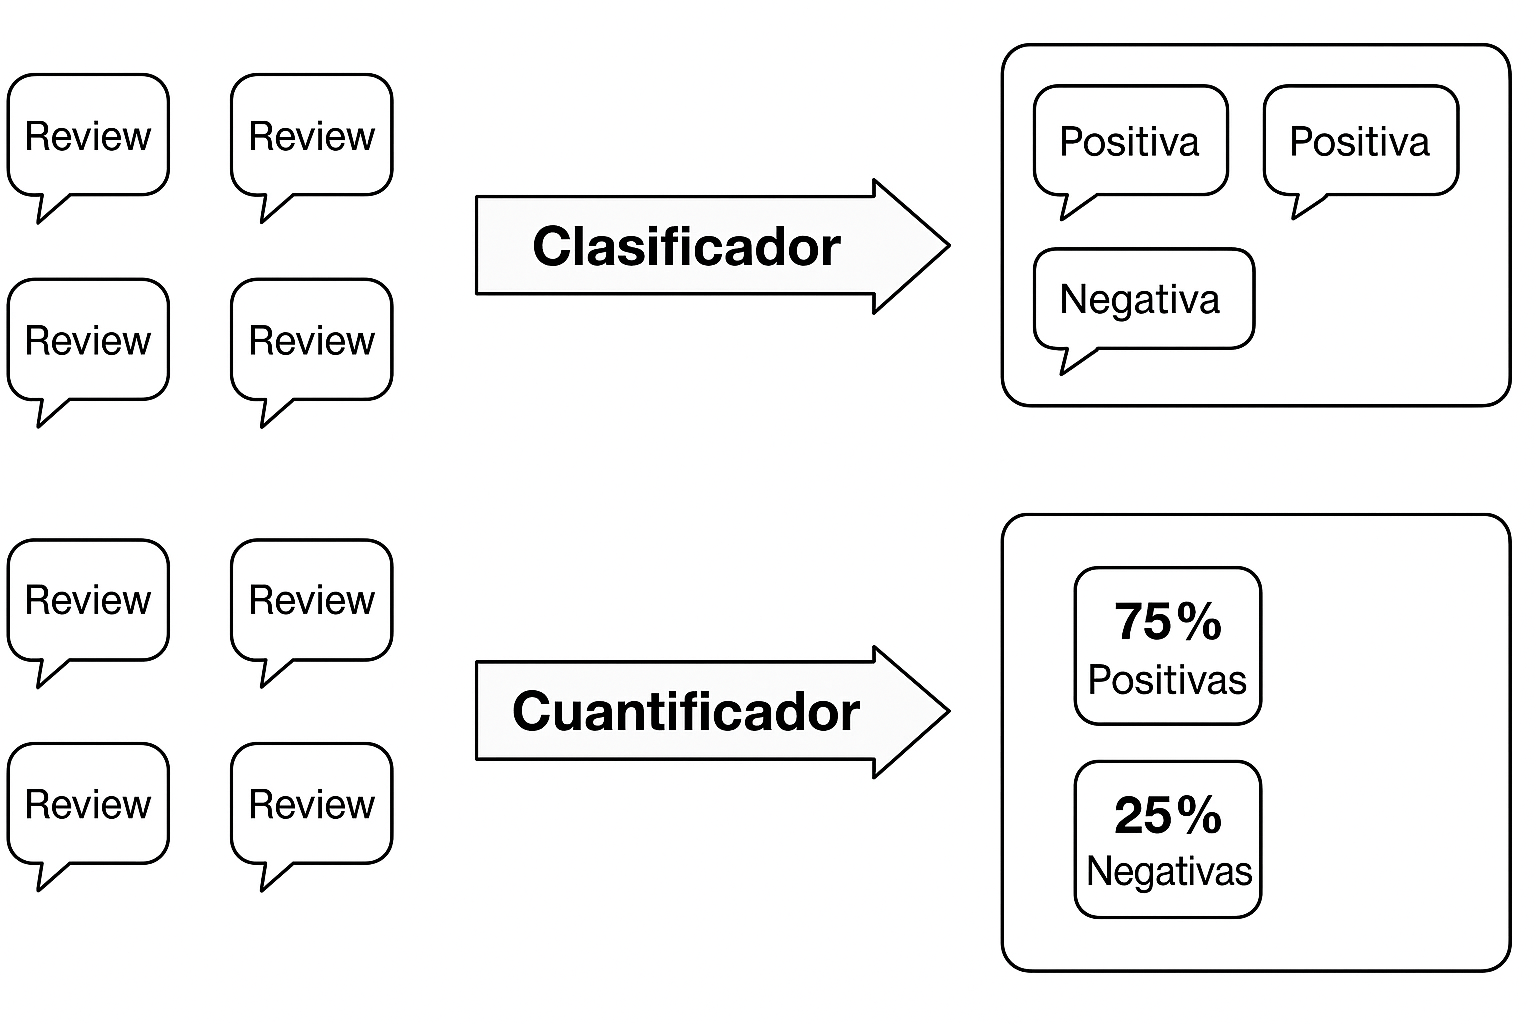
\includegraphics[scale=0.13]{images/quantificaiton.png}
\end{frame}

\begin{frame}{Asunción de cambio de distribución}
\begin{columns}
    \begin{column}{0.5\textwidth}
        \begin{itemize}
            \item Suponemos que existe un \textbf{cambio de distribución} entre los datos de entrenamiento y los de test, concretamente \textbf{Prior Probability Shift}:
            \begin{equation}
                p_{\text{train}}(x \mid y) = p_{\text{test}}(x \mid y)
            \end{equation}
            \begin{equation}
                p_{\text{train}}(y) \neq p_{\text{test}}(y)
            \end{equation}
            \item Es decir: cambia la prevalencia de las clases, pero no el concepto de cómo son los ejemplos de cada clase.
        \end{itemize}
    \end{column}
    \begin{column}{0.1\textwidth}
    \end{column}
    \begin{column}{0.4\textwidth}
        \centering
        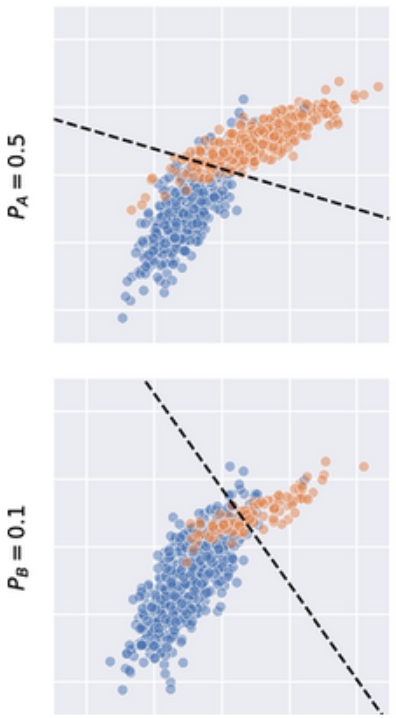
\includegraphics[width=\linewidth]{images/pps.png} 
    \end{column}
\end{columns}
\end{frame}

% 3. Dataset
\begin{frame}{Dataset: Amazon Reviews (LeQua)}
\begin{itemize}
    \item Opiniones de productos en Amazon.
    \item Dos clases: \textbf{positivas} y \textbf{negativas}.
    \item Se han preprocesado y convertido a vectores con 250 características por cada opinión (bag-of-words o embeddings).
    \item Conjunto de entrenamiento etiquetado individualmente con \textbf{5000 opiniones}.
    \item Conjunto de validación para probar nuestros cuantificadores con \textbf{1000 bolsas} con \textbf{250 opiniones} cada una.
    \begin{itemize}
        \item Cada bolsa contiene un conjunto de opiniones con una distribución concreta de clases.
        \item No disponemos de las etiquetas individuales de cada opinión.
    \end{itemize}
\end{itemize}
\begin{block}{Opinión positiva}
    \small
    \emph{“Me encanta este producto, llegó rápido y es de muy buena calidad. Lo recomiendo sin duda.”}
    \end{block}
    
    \begin{block}{Opinión negativa}
    \small
    \emph{“El producto no funcionaba, muy mala experiencia. No lo volveré a comprar.”}
    \end{block}
\end{frame}


% 4. Quantificationlib
\begin{frame}{¿Qué es quantificationlib?}
\begin{itemize}
    \item Librería Python para cuantificación: \url{https://github.com/AICGijon/quantificationlib}
    \item Proporciona implementaciones de los cuantificadores más relevantes:
    \begin{itemize}
        \item \textbf{CC}: Classify \& Count (solución trivial).
        \item \textbf{AC}: Adjusted Count.
        \item \textbf{DFy}: Métodos basados en ajuste de distribuciones.
        \item \textbf{EMQ}: Expectation Maximization.
        \item ...
    \end{itemize}
    \item Permite entrenar y evaluar cuantificadores de forma sencilla.
\end{itemize}
\centering
%add vertical space
\vspace{0.5cm}

\includegraphics[width=0.6\linewidth]{images/python.png}
\end{frame}

\begin{frame}{¡Manos a la obra!}
\centering
\huge
\url{http://bit.ly/44uRwag}
\end{frame}

\end{document}
